\setAuthor{Mihkel Kree}
\setRound{piirkonnavoor}
\setYear{2017}
\setNumber{G 9}
\setDifficulty{6}
\setTopic{Elektrostaatika}

\prob{Laengud}
\begin{wrapfigure}{r}{0.3\textwidth}
	\vspace{-25pt}
	\begin{center}
		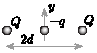
\includegraphics[width=0.32\textwidth]{2017-v2g-09-laengudjoonis.pdf}
	\end{center}
	\vspace{-10pt}
\end{wrapfigure}

Kaks kera, kumbki laenguga $Q$, on liikumatult fikseeritud nii, et nende keskpunktide kaugus on $2d$. Täpselt nende kerade keskele paigutatakse kolmas kera laenguga $-q$ ning massiga $m$, mis saab liikuda ainult mööda $y$-telge (vt joonis). Leidke selle kolmanda kera väikeste $y$-suunaliste võnkumiste periood $T$.

\hint
Väikeste $y$-suunaliste võnkumiste jaoks on kasulik vaadata, missugune jõud kerale mõjub, kui seda väikse distantsi $y$ võrra tasakaaluasendist eemale nihutada.

\solu
Olgu keskmise kera nihe $y$. Keskmise kera kaugus kummastki äärmisest kerast on nüüd $l=\sqrt{d^2+y^2}$. Kumbki äärmine kera mõjutab keskmist kera jõuga $F=\frac{kqQ}{l^2}$, mille vertikaalkomponent on $F_y=-\frac{y}{l}F$. Kokku mõjub keskmisele kerale vertikaaljõud $2F_y$, millest saame seose keskmise kera kiirenduse jaoks $ma=2F_y$. Et $y\ll d$, siis $l\approx d$, millest saame lihtsustada liikumisvõrrandi kujule
\[
a=-\frac{2kQq}{md^3}y.
\]
See võrrand kirjeldab harmoonilist võnkumist perioodiga 
\[ T = 2\pi \sqrt{\frac{md^3}{2kQq}}.\]
{\em Märkus.} perioodi ja sageduse valem on võimalik leida analoogiast vedru võnkumisega, kus $ma = -kx$ ja $T=2\pi \sqrt{m/k}$.

\probeng{Charges}
\begin{wrapfigure}{r}{0.3\textwidth}
	\vspace{-25pt}
	\begin{center}
		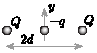
\includegraphics[width=0.32\textwidth]{2017-v2g-09-laengudjoonis}
	\end{center}
	\vspace{-10pt}
\end{wrapfigure}
Two balls, each with a charge $Q$, are firmly fixed so that the distance between their centers is $2d$. A third ball with a charge $-q$ and mass $m$ is placed exactly in the middle of the two balls. The third ball can only move along the $y$-axis (see figure). Find the period $T$ of the third ball’s small oscillations along the $y$-axis.

\hinteng
For small $y$-directional oscillations it is useful to look what sort of force is applied to the ball if it is moved away from the equilibrium position by a small distance $y$.

\solueng
Let the displacement of the middle ball be $y$. The distance of the middle ball from both of the outer balls is now $l=\sqrt{d^2+y^2}$. Both of the outer balls apply a force $F=\frac{kqQ}{l^2}$ to the middle ball, the vertical component of that force is $F_y=-\frac{y}{l}F$. The total force applied to the middle ball is $2F_y$ from which we get a relation for the middle ball’s acceleration: $ma=2F_y$. Since $y\ll d$ then $l\approx d$ from which we can simplify the equation of motion into
\[
a=-\frac{2kQq}{md^3}y.
\] 
This equation describes a harmonic oscillation with a period
\[ T = 2\pi \sqrt{\frac{md^3}{2kQq}}.\] 
\emph{Note}. The formula of period and frequency is possible to find the same way as the spring’s oscillation where $ma = -kx$ and $T=2\pi \sqrt{m/k}$.
\probend